\documentclass[12pt, titlepage]{article}

\usepackage{fullpage}
\usepackage[round]{natbib}
\usepackage{multirow}
\usepackage{booktabs}
\usepackage{tabularx}
\usepackage{graphicx}
\usepackage{float}
\usepackage{hyperref}

\hypersetup{
    colorlinks,
    citecolor=black,
    filecolor=black,
    linkcolor=black,
    urlcolor=blue
}
\usepackage[round]{natbib}

\title{SE 3XA3: Test Report\\Snake 2.o}

\author{Team \#30, VUA30
		\\ Usman Irfan - irfanm7
		\\ Andy Hameed - hameea1
		\\ Vaibhav Chadha - chadhav
}

\date{\today}

\begin{document}

\maketitle

\pagenumbering{roman}
\tableofcontents
\listoftables
\listoffigures

\begin{table}[bp]
\caption{\bf Revision History}
\begin{tabularx}{\textwidth}{p{3cm}p{2cm}X}
\toprule {\bf Date} & {\bf Version} & {\bf Notes}\\
\midrule
2018-12-04 & 1.0 & Andy worked on 5 - how Intergrated \& System testing helped the process \\
2018-12-05 & 1.0 & Usman worked on Functional Requirements \& tracing the requirements to the test \\
2018-12-05 & 1.0 & Vaibhav worked on section 2,3 and 9\\
\bottomrule
\end{tabularx}
\end{table}


\newpage

\pagenumbering{arabic}



\section{Functional Requirements Evaluation}
\begin{enumerate}
	\item{\textbf{TID1}\\}
	Test Result: 
	The requirement was successfully completed by clicking the three levels of the game and the tester saw a transition from the main menu to the Theme
	interface. PASSED.

	\item{\textbf{TID2}\\}
	Test Result:
	The requirement was successfully completed by clicking the three distinct themes the game has to offer and the tester saw a transition from the main menu
	to the Gameplay interface where the background color and snake color changed to its respective theme. PASSED.

	\item{\textbf{TID3}\\}
	Test Result:
	The tester can open a see the highest score of the game by clicking on the button Highscore from the main menu, this was tested by playing the game and notice that after making a new highest score the score was updated in the Highest Screen page. PASSED.


	\item{\textbf{TID4}\\}
	Test Result:
	Once the user is in the gameplay. The initial movement of the snake could arbitrary, this was tested by playing the game four times and tested all the directional key works as the first move. PASSED.

	\item{\textbf{TID5}\\}
	Test Result:
	The game was played multiple times and kept track that the initial location of the snake changes every time. PASSED.


	\item{\textbf{TID6}\\}
	Test Result:
	When the snake eats the food the food's location was updated on the screen and was displayed randomly. To meet this requirement we additionally tested the game so the food doesn't appear inside the snake's body or outside the screen. PASSED.

	\item{\textbf{TID7}\\}
	Test Result:
	The directional key was tested by pressing the UP key, the snake moved one-unit up to the respective direction. PASSED.

	\item{\textbf{TID8}\\}
	Test Result:
	The directional key was tested by pressing the DOWN key, the snake moved one-unit up to the respective direction. PASSED.

	\item{\textbf{TID9}\\}
	Test Result:
	The directional key was tested by pressing the LEFT key, the snake moved one-unit up to the respective direction. PASSED.

	\item{\textbf{TID10}\\}
	Test Result:
	The directional key was tested by pressing the RIGHT key, the snake moved one-unit up to the respective direction. PASSED.

	\item{\textbf{TID11}\\}
	Test Result:
	The requirement was successfully completed by clicking the three distinct levels the game has to offer, the differences that each level had was visualized and their speed increased as levels increased (except the intermediate and advanced had the same speed, as planned in the requirement). In the easy mode, the snake could cross the boundaries. In the intermediate stage, the snake dies when it tries to cross the boundary. In the advanced stage, the snake dies when it tries to cross the boundary or touches the maze. PASSED.

	\item{\textbf{TID12}\\}
	Test Result:
	The snake would never die before eating food at an easy level. The only way to die is for the snake to eat itself. PASSED.

	\item{\textbf{TID13}\\}
	Test Result:
	When the snake dies there is a transition in the page which tells the user to play the same again, go to the Main Menu or Quit. This transition was observed and all three options worked. PASSED.



\end{enumerate}
\section{Nonfunctional Requirements Evaluation}

The following tests are performed using the Test Plan. Please refer to that document to get the test ID's.
\subsection{Look and Feel}
\begin{enumerate}
	
	\item{\textbf{TID14}\\}
	
	Test Result: For this test, the application was run and it was observed the application launches with an interface. This interface met the requirements of the game. PASSED.
	
\end{enumerate}

\subsection{Usability}

\begin{enumerate}
	
	\item{\textbf{TID15}\\}
	
	Test Result: Usability of the application was tested by asking people of different ages to play this game. Then, they were asked to fill a survey on Google forms where they selected their age and user-friendliness of the program. After running the test, an average of 4.5 out of 5 was achieved. PASSED
	
\end{enumerate}

\subsection{Performance}
\begin{enumerate}
	
	\item{\textbf{TID16}\\}
	
	Test Result: Dynamic testing was performed to do this task. For this various buttons were pressed and the delay time was observed. Every time, the application was able to respond fairly quickly. PASSED
	
	\item{\textbf{TID17}\\}
	
	Test Result: In order to perform this testing, different modes of the game were played and the speed difference was observed. Also, it was observed teh the snake speed doesn't change itself and remains constant within a level. For example, there was quite a seed difference between beginner and intermediate. PASSED
	
	\item{\textbf{TID18}\\}
	
	Test Result: A group of people were asked to play this game and check the responsiveness of buttons while playing the game. After performing this Beta Testing, we got an average rating of 4.7 out of 5 for this area which gives this a clear pass. PASSED
	
\end{enumerate}

\subsection{Operational and Environmental}
\begin{enumerate}
	
	\item{\textbf{TID19}\\}
	
	Test Result: While asking different people to play this game, USB was used as a resource to transfer this. 100\% of the time, the game was able to run on the other device. PASSED
	
\end{enumerate}

\subsection{Maintainability and Support Requirements}
\begin{enumerate}
	
	\item{\textbf{TID20}\\}
	
	Test Result: When the group of individuals were asked to take a part in our Beta Testing of the game, every user had a device of their own choice. Overall, the group consisted of people with Windows, Mac OD and Linux operating devices. The software was able to run completely fine on all of them. PASSED
	
\end{enumerate}

\subsection{Security and Cultural}
\begin{enumerate}
	
	\item{\textbf{TID21}\\}
	
	Test Result: This software does not contain any outside source of information except the snake logo. The snake logo was taken from an open source website allowing us to use it for any non-commercial purpose. Also, the game checked several times to make sure that the game does not contain anything illegal or offensive. PASSED
	
\end{enumerate}

\section{Comparison to Existing Implementation}	

This game is inspired from an old game made by Patrick Gillespie in JavaScript. The current implementation is done using python and making some improvements over the existing game. The interface is one of the major improvements of this project. The old interface has everything (levels, high score, playground) clustered onto one page whereas we implemented them in different modules. Also, numerous features were added such that snake going through boundary in beginner and additional barrier in advances mode. Also, a help page was added to the implementation in order to help new players. Overall, this project extends the existing implementation really well and provide the user with a really fun experience.

\section{Unit Testing}

Due to the nature of the project, manual and integrated/system testing will be performed throughout the development process to check for correctness and verify adherence to functional and nonfunctional requirements.

In future implementations, it may be possible to apply unittests but with the current implementation of the software, a complete reimplementation would be required in order to create unit test cases. The assert statements available will not help with testing the gameplay since the game itself runs within the 1 main function that controls that game, the game() function in the Gameplay module. This means that within the while loop, the local variables and snake state variables are changing and there is no checkpoint to use in the assert statements since this all happens in the middle of a function call, in an infinite while loop (until the user dies).

\section{Changes Due to Testing}
Through integrated and system testing, which encompassed the majority of the testing done on the software, the user interface as well as bugs and errors in the gameplay were modified to fix erroneous properties of the software. By continuously executing the game, it was easy to estimate changes in object coordinates within the interface. For example, the menu buttons were arranged through trial and error by testing the software continuously until the desired look was acheived. Beyond that, system and intergrated testing confirmed that all modules were working correctly and any change in one of the modules did not affect the function of other modules through dependency relations.

Similarly, the gameplay was tested and verified by the developers of the software as well as peers and classmates to ensure proper functioning. Through feedback received in the google survey, errors and modifications were made: For example, one user suggested an excitement element to be added to the game and a maze feature was added to the advanced difficulty gameplay mode to accomodate for that. As seen in Figure 1, feedback received from peers included both functional and non-functional properties and aided in the software revision process.

\begin{figure}
  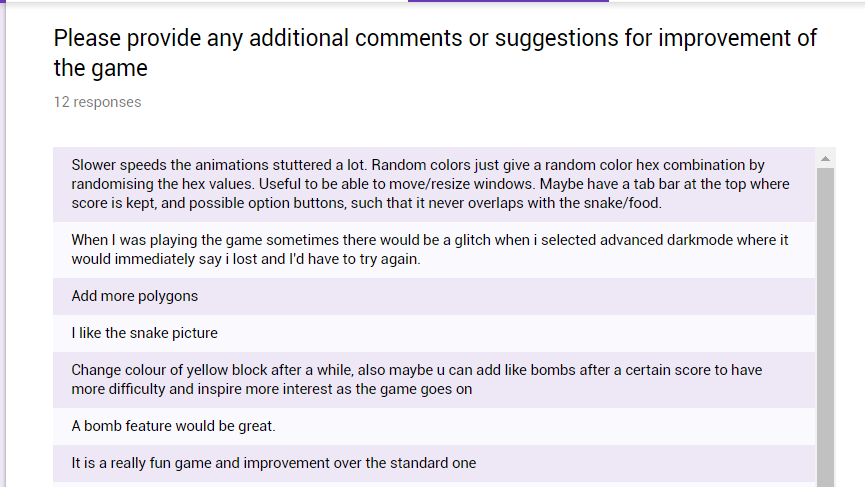
\includegraphics[width=\linewidth]{feedback.png}
  \caption{Peer Feedback \& Comments}
\end{figure} 

\section{Automated Testing}
The main testing for this program was done through dynamic testing whcih has been discussed in the requirements. The validation
for the testing of the product was done by peer review, surveys and self-testing. Boundary cases and groups of test cases were used in dynamic testing to visualize the output and fix it.
\section{Trace to Requirements}
To meet the functional and non-functional requirements for the program, the requirements were divided into groups and modular
were created for each group. A module for the high score part was made in which the requirements for displaying the highest score, displaying the highest score and storing it was done.\\
Moreover, a theme module was made to meet the requirements regarding the selection of the theme. The user could select two types of themes from the main menu and then the gameplay would have a background of that color, with different themes the color of the snake changes.\\
To focus on the major requirements, most of the requirements were accomplished in the Gameplay and Interface module. Gameplay module was responsible for all the code in the backend. Requirements controlling the snake, altering the speed for the snake, checking boundary conditions for each level in the game was done in this module.\\
The interface module is more focused on the frontend, it visualizes the backend program to a user-interface which increases usability and allow the user to communicate with the program easily.ted for each group. A module for the highscore part

% the table should use mref, the requirements should be named, use something
% like fref
\begin{table}[H]
\centering
\begin{tabular}{p{0.2\textwidth} p{0.6\textwidth}}
\toprule
\textbf{Req.} & \textbf{Modules}\\
\midrule
FR1 & M2, M5\\
FR2 & M5, M9\\
FR3 & M2, M8\\
FR4 & M7, M9\\
FR5 & M7, M9\\
FR6 & M9\\
FR7 & M7, M9\\
FR8 & M7, M9\\
FR9 & M7, M9\\
FR10 & M7, M9\\
FR11 & M9\\
FR12 & M9\\
FR13 & M9, M2, M5, M8\\

\bottomrule
\end{tabular}
\caption{Trace Between Requirements and Modules}
\label{TblRT}
\end{table}

\begin{table}[H]
\centering
\begin{tabular}{p{0.2\textwidth} p{0.6\textwidth}}
\toprule
\textbf{AC} & \textbf{Modules}\\
\midrule
AC1 & M1\\
AC2 & M2, M6\\
AC3 & M6\\
AC4 & M5,M6\\
AC5 & M6\\
AC6 & M5\\
AC7 & M2\\
\bottomrule
\end{tabular}
\caption{Trace Between Anticipated Changes and Modules}
\label{TblACT}
\end{table}

\section{Trace to Modules}		
Integrated testing can visibly be traced back to the modules created. The main interface uses the Interface module along with GUI module for interface text and buttons. It is connected to the highscore module and theme module through the highscore and difficulty level buttons respectively. It also connected to the help module through the Help button. If any of these buttons is clicked and an error is released, the error can be traced back with ease depending on the button that was clicked prior to the malfunction.

	This same pattern is applied in the theme module, between the regular, dark and random modes. Each button corresponds to color and setup parameters that reflect the chosen theme. If a specific them is not working, it can be traced back in the theme module through the commented blocks of code corresponding to each respective theme. 

	In the gameplay module, testing can be traced back based on user action and system response. Through the use of commenting it is visible to identify particular functionality such as snake direction change, detection of barrier collisions, snake body collisions, collision with a food block and so on. The traceability of malfunctioning parts within the actual game can be traced back within the gameplay module, which encompasses all functionality under which the snake game operates. 

\section{Code Coverage Metrics}

The VUA 30 group has managed to produce anywhere between 95 to 100 percent of code coverage through the tests. This number is highly based on the fact that each of the modules has been covered by the testing. Each test and the results have been recorded in this document which highly matches with the expected results from the Test Plan.  Please refer to the TID's above and trace to modules in order to follow up with the testing. Finally, this clearly shows that the group has been able to cover the majority of the aspects of this project, once again confirming the high percent coverage rate.

\bibliographystyle{plainnat}



\end{document}